\documentclass[10pt]{beamer}

\usetheme[progressbar=frametitle]{metropolis}
\usepackage{appendixnumberbeamer}

\usepackage{booktabs}
\usepackage[scale=2]{ccicons}
\usepackage{multimedia}
\usepackage{wrapfig}
\usepackage{tabularx}
\usepackage{esint}
\usepackage{amsmath}

\usepackage{pgfplots}
\usepgfplotslibrary{dateplot}

\usepackage{xspace}
\newcommand{\themename}{\textbf{\textsc{metropolis}}\xspace}

\title{Vibration Suppression Design for Virtual Compliance Control in Bilateral Teleoperation}
% \date{\today}
\date{}
\author{Edoardo Ghini, Gianluca Cerilli, Giuseppe L'Erario}
\institute{La Sapienza University}
% \titlegraphic{\hfill\includegraphics[height=1.5cm]{logo.pdf}}

\begin{document}
	
	\maketitle
	
	\begin{frame}{Table of contents}
	\setbeamertemplate{section in toc}[sections numbered]
	\tableofcontents[hideallsubsections]
\end{frame}

\section{Introduction}

\begin{frame}[fragile]{Problem statement}

Application of one degree of freedom inertia-spring-damper system for \textbf{vibration suppression} in a bilateral control system.\\
\bigskip
System compliance for different input frequency controlled by the
value of virtual elements (based on the cut-off frequencies and stiffness of the virtual spring).

\end{frame}
\begin{frame}[fragile]{Motivation}

\begin{enumerate}
\item \textbf{Stability} of the closed loop system irrespective to the behaviour of the human and the environment
\bigskip
\item \textbf{Transparency} of the teleoperation task: same forces and displacements on the two sides of the system \end{enumerate}

\end{frame}

\section{System Modeling}

\begin{frame}{Inertia-Spring-Damper System}
	
	\begin{figure}[h]
	\centering
	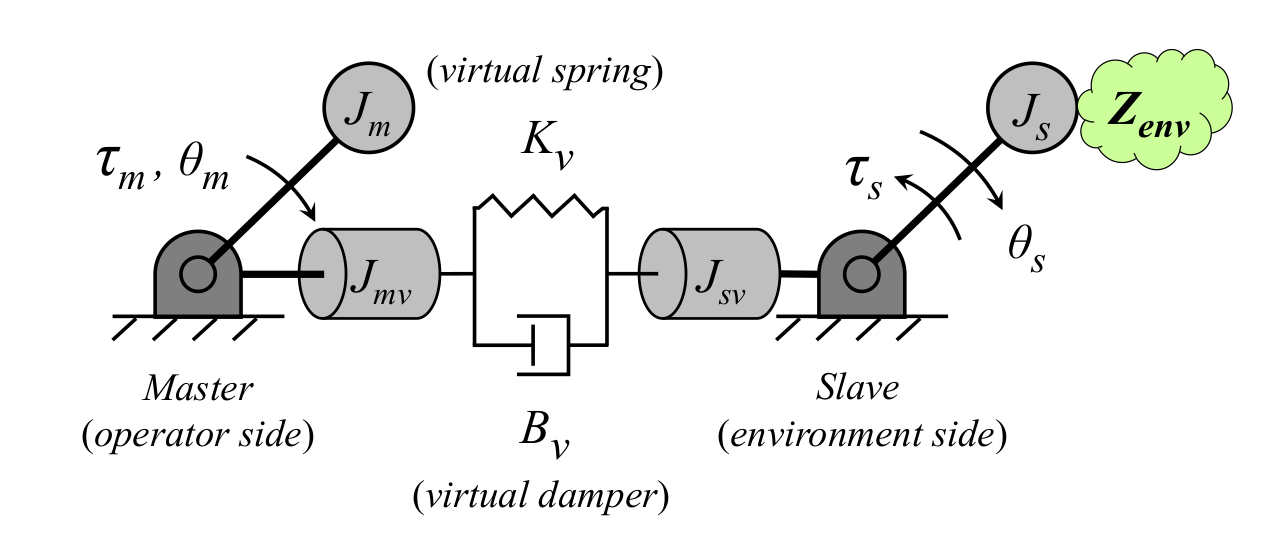
\includegraphics[width=0.8\linewidth]{../../../../QuadrotorModelling/TELEOPERATION/reportTeleop/Images/spring_damper_inertia_system}
	\end{figure}

Position error based torque reflection to the operator at the
master side.
	
	\begin{list}{$ \circ $}{}
		\item Real inertias: $ J_{m}, J_{s} $
		\item Virtual inertias: $ J_{mv}, J_{sv} $
		\item Virtual damper and spring: $ B_{v}, K_{v} $
	\end{list}

\end{frame}

\begin{frame}{Bilateral Control Scheme}

	\begin{figure}
	\centering
	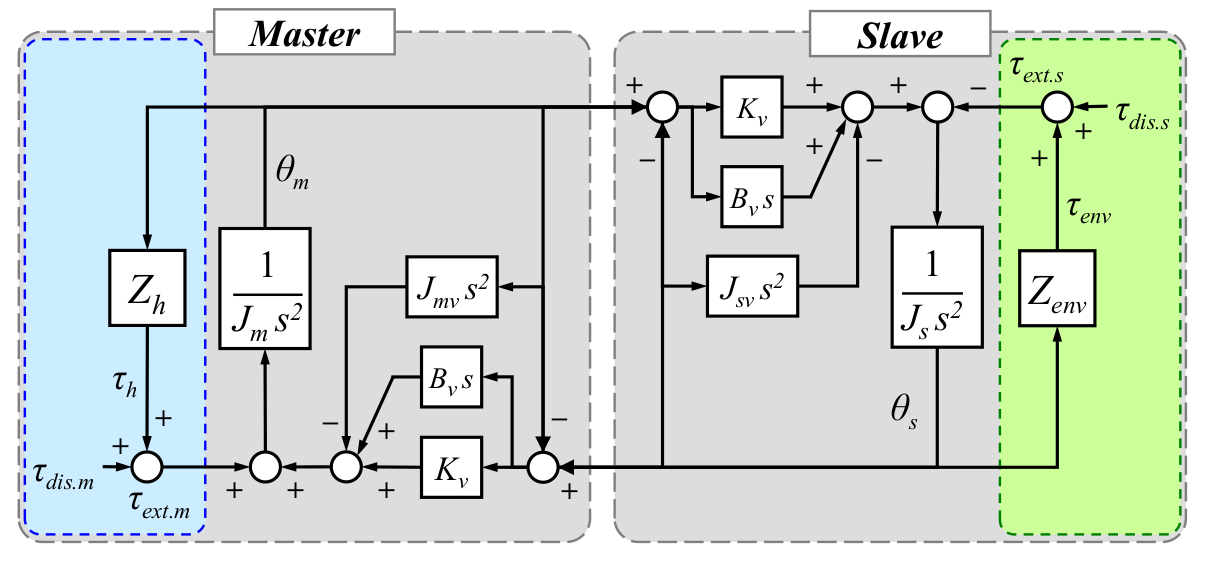
\includegraphics[width=0.8\linewidth]{../../../../QuadrotorModelling/TELEOPERATION/reportTeleop/Images/Block_diagram}
	\end{figure}

Dynamics equations in frequency domain:
\begin{align*}
	(J_m + J_{mv}) s^2 \theta_m + (B_v s + K_v) (\theta_m - \theta_s) &= \tau_m \\
	(J_s + J_{sv}) s^2 \theta_s + (B_v s + K_v) (\theta_s - \theta_m) &= -\tau_s 
\end{align*}
	
\end{frame}

\section{System Analysis}

\begin{frame}[fragile]{Bilateral Controller}

External torques as action and reaction torque of human and environment impedance, $ Z_{h} $ and $ Z_{env} $:
\begin{align*}
	J_m s^2 \theta_m &= \tau_m - (B_v s + K_v) (\theta_m - \theta_s) - J_{mv} s^2 \theta_m \\
	J_s s^2 \theta_s &= - \tau_s - (B_v s + K_v) (\theta_s - \theta_m) - J_{sv} s^2 \theta_s
\end{align*}

System represented by 2$\times $2 hybrid matrix as:

\begin{equation*}
\begin{bmatrix}
\tau_m \\ \theta_s
\end{bmatrix} = 
\begin{bmatrix}
H_{11} & H_{12} \\
H_{21} & H_{22}
\end{bmatrix}
\begin{bmatrix}
\theta_m \\ - \tau_s
\end{bmatrix}
\label{hybrid_matrix}
\end{equation*}

\end{frame}

\begin{frame}[fragile]{Bilateral Controller}

Hybrid parameters $ H_{ij} $:
\begin{align*}
	H_{11} &= \frac{1}{Z_s}[Z_m Z_s - (B_v s + K_v)^2] \\
	H_{12} &= -\frac{1}{Z_s}[B_v s + K_v] \\
	H_{21} &= \frac{1}{Z_s}[B_v s + K_v] \\
	H_{22} &= \frac{1}{Z_s} 
\end{align*}
where:
\begin{align*}
	Z_m &= (J_m + J_{mv}) s^2 + B_v s + K_v \\
	Z_s &= (J_s + J_{sv}) s^2 + B_v s + K_v
\end{align*}

\end{frame}

\begin{frame}{Bilateral Controller}

\textit{Condition of transparency}: Trasmitted impedance $ Z_{t} $ transferred to the operator should be equal to environment impedance $ Z_{env} $:
\begin{equation*}
	\frac{\tau_m}{\theta_m} = Z_t = Z_{env} = \frac{\tau_s}{\theta_s}
\end{equation*}
Relationship between $ Z_{t} $ and $ Z_{env} $:
\begin{equation*}
	Z_t = \big(\dfrac{-H_{12} H_{21}}{1 + H_{22} Z_{env}}\big)Z_{env} + H_{11}
\end{equation*}
Hybrid parameters for the perfect transparency condition, derived as:
\begin{equation*}
	\begin{bmatrix}
	\tau_m \\ \theta_s
	\end{bmatrix} = 
	\begin{bmatrix}
	0 & -1 \\ 1 & 0
	\end{bmatrix}
	\begin{bmatrix}
	\theta_m \\ -\tau_s
	\end{bmatrix}
\end{equation*}

\end{frame}

\section{Vibration Suppression Design}

\begin{frame}{Parameters Selection and Design}

Assume system disturbed by environment vibration noise.\\
\bigskip
Inspect $ H_{22} $ for the relationship of position response $ \theta^{res} $ and external torque input $ \tau_{ext} $:
\begin{equation*}
	\dfrac{\theta_s}{\tau_{ext}} = \dfrac{1}{(J_s + J_{sv}) s^2 + B_v s + K_v}
	\label{H_22}
\end{equation*}\\
\bigskip
Virtual parameters $ J_{v}, B_{v} $ and $ K_{v} $ determined from the second-order characteristic equation:
\begin{equation*}
	s^{2} + (g_{1} + g_{2})s + (g_{1}*g_{2}) = 0
\end{equation*}
established from two poles $ g_{1} $ and $ g_{2} $, representing the desired cut-off frequencies of the system for disturbance suppression.

\end{frame}

\begin{frame}{Parameters Selection and Design}
	
Spring stiffness $ K_{v} $ influences the behaviour of the system.\\
\bigskip
It regulates the \textit{compliance} of this, achieving \textbf{rigid coupling} (high spring stiffness) or \textbf{spring coupling} (low spring stiffness).\\
\bigskip
Virtual parameters $ B_{v} $ and $J_{v} $ computed according to $ K_{v} $:
\begin{equation*}
	B_v = \left(\frac{g_1 + g_2}{g_1*g_2}\right) K_v
\end{equation*}
and
\begin{equation*}
	J_{sv} = \left(\frac{1}{g_1*g_2}\right) K_v - J_s
\end{equation*}

\end{frame}	

\begin{frame}{Vibration Suppression Performance Analysis}
	
	
	
\end{frame}	

\section{Results}

\begin{frame}{Simulation Setup}

\end{frame}

\begin{frame}{Simulation Scenario and Results}
	
\end{frame}

\begin{frame}{Simulation Scenario and Results}
	
	VIDEO
	
\end{frame}

\section{Conclusion}

\begin{frame}{Summary}

\end{frame}

{\definecolor{BlueTOL}{HTML}{222255}
\setbeamercolor{palette primary}{fg=black, bg=white}
\begin{frame}[standout]
Thank you for your attention!
\end{frame}
}

\appendix

\end{document}
